
\chapter{
Le soufisme ou la mystique en islam}


\section{Calligraphie}


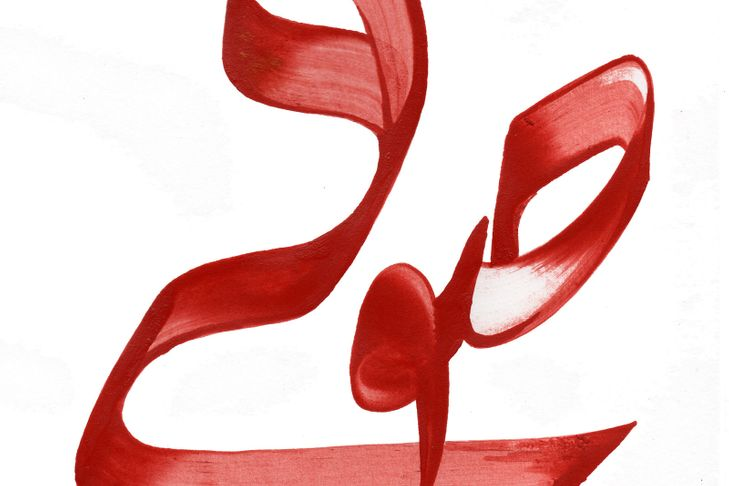
\includegraphics[width=\textwidth]{Images/image013.jpg}


« Aux commencements de l'islam, il n'y a ni ascètes ni soufis.
L'ascétisme et la mystique musulmane vont se développer dans les
sociétés de convertis à partir du IX\textsuperscript{e}~siècle. C'est un
phénomène d'hybridation culturelle. Le soufisme est d'abord le fait de
maîtres isolés au IX\textsuperscript{e}~siècle, vivant du côté de
l'actuel Iran. À partir du XII\textsuperscript{e}~siècle se développent
les premières confréries, dont certaines sont encore vivantes
aujourd'hui. Dans l'islam, la mystique est aussi développée que dans le
christianisme, mais elle a été davantage combattue. D'abord par les
juristes, qui voyaient d'un mauvais œil ces croyants qui s'émancipaient
des règles sociales, puis par le wahhabisme, qui les a massacrés dans la
deuxième­ moitié du XVIII\textsuperscript{e}~siècle ».\sn{Jacqueline Chabbi}


« Dans cette calligraphie, j'ai recherché la stabilité mais aussi un
geste plus tendre. Certains y verront peut-être un personnage
agenouillé, en prière\ldots{} Pourquoi pas ? J'offre une image sur
laquelle je ne peux pas toujours mettre des mots. C'est à ceux qui
regardent d'interpréter mes images. Quand je peins, je prends toujours
en considération le blanc laissé par la trace. En calligraphie, un
principe dit :\emph{~``Le noir de votre calligraphie, c'est vous. Le
blanc de votre calligraphie, c'est vous aussi.''}~J'y pense souvent.
Dans les textes anciens, le soufi -- que l'on peut traduire par
``mystique'' -- doit travailler sur soi-même pour retrouver la lumière
intérieure. Il devient alors pur et peut arriver à rencontrer la
divinité. »\sn{Hassan Massoudy}
\section{Introduction}
Qu'est-ce que le soufisme~? Pour les soufis, il s'agit de la dimension
spirituelle et originelle de l'islam. Le mot originel est important~: il
signifie que le soufisme est connaturel à l'islam, qu'il est l'islam. Il
ne s'agit pas d'un développement ultérieur qui aurait eu lieu sous
l'influence du monachisme chrétien ou du šī`isme, mais de l'islam vécu
par Muḥammad et ses compagnons. Donc, pour les soufis, Muḥammad est un
soufi. Les salafs, les anciens, les compagnons de Muḥammad sont soufis.
On comprend que si al-Ġazālī \label{theol:AlGazali27} considère le soufisme comme la voie par
excellence pour aller à Dieu, il n'en demeure pas moins que sous sa
plume la référence aux salafs y est importante.
\mn{Le soufisme et Si'isme

\begin{itemize}
\item
  historiquement, plutôt dans l'islam sunnisme
\item
  dans le si'isme, c'est presque intégré tellement il est naturellement
  spirituel.

  \item
    Dans le cadre duodecimain strict, on ne prie pas les imams
  \item
    Mais en fait, il y a des «~sectes~» qui vont le prier, à commencer
    par le fait qu'on va considérer que c'est le «~l'imam caché~»

  \end{itemize}}
Pour autant, cette affirmation d'éminents soufis n'est pas partagée par
l'ensemble des penseurs de l'islam, et au cours de l'histoire, le
soufisme a pu faire l'objet de critiques, de contestations, de
réfutations plus ou moins virulentes. Certaines des pratiques soufies
ont pu être considérées comme hétérodoxes, innovatrices, non conformes à
l'islam des origines. Ce sont ces accusations récurrentes qui permettent
d'expliquer pourquoi on s'en prend aujourd'hui encore à des mosquées
soufies. Le wahhabisme est la matrice idéologique anti-soufie
contemporaine. Comme nous l'avons vu, il est né en Arabie à partir du
18\textsuperscript{ème} siècle en contestant les confréries soufies
jugées non confirmes à l'islam. Aujourd'hui, l'État islamique de l'Irak
et du Levant, au lendemain de la conquête de Mossoul a distribué aux
habitants une charte comprenant 16 commandements~: à l'article 10, il
est écrit que toutes les manifestations publiques contraires à l'islam
sont interdites (article 10). En 2014, quatre sanctuaires sunnites et
soufis et six mosquées chiites ont été détruites dans la province de
Ninive, sous contrôle des insurgés. La destruction la plus spectaculaire
fut celle du tombeau du prophète Jonas -- Yunus en arabe -- qui a été
réduite à un amas de cailloux.

En Égypte, dans le Sinaï, en décembre 2016, un shaykh soufi et un de ses
disciples sont assassinés par le groupe de l'Etat islamique. Le 24
novembre 2017 l'attentat à la mosquée al-Rawdah de Bir al-Abed fait 305
morts -- à cette mosquée était attachée une \emph{zāwiya} -- édifice
religieux fréquenté par des soufis et des conscrits de l'armée. Cette
mosquée soufie appartient à l'ordre soufi des ǧarirites du nom d'Aïd Abū
Ǧarīr qui a fondé trois loges dans le Sinaï au 20\textsuperscript{ème}
siècle dont celle de Bir al-Abed\sn{Sur la sociologie religieuse
  du Sinaï, voir l'article d'Ismaïl Alexandrani~:
   \url{http://orientxxi.info/magazine/-genealogie-du-djihadisme-au-sinai,0687}}.

\vide{i--duxe9finir-le-soufisme}{%
\section{{Définir le soufisme
}}\label{i--duxe9finir-le-soufisme}}

En guise d'apéritif, écoutez la voix d'Henri Corbin (m. 1978),
philosophe et éminent orientaliste français, spécialiste surtout de
l'islam iranien et de la gnose chiite. \emph{Extrait d'un entretien avec
Bernard Maxime Latour en 1971}.

Définition complexe donc, «~tâche scabreuse~»\ldots{} essayons cependant
de le définir à partir de la manière dont les musulmans eux-mêmes
présentent le soufisme, le \emph{tasawwuf} en arabe.

Pour cela, je vous propose de lire un extrait du livre Traité de
Kalābāḏī, \emph{Kitāb al-ta`arruf li-maḏhab ahl al-tasawwuf} qui a été
traduit par Roger Deladrière\sn{~\textsc{Kalābāḏī}, \emph{Kitāb
  al-taʿarruf li-madhhab ahl al-taṣawwuf} {[}traduction française~:
  Traité de soufisme, Les Maîtres et les étapes, traduit de l'arabe et
  présenté par Roger Deladrière, Paris, Actes-Sud, Sinbad, 1981.}.
Kalābāḏī \label{theol:Kalabadi} est un auteur persan, mort aux environs de 990. Cet ouvrage
cherche à réconcilier le soufisme et l'orthodoxie. C'est un classique,
apprécié de tous. En son introduction, il consacre plusieurs pages à
cerner le sens de soufisme par l'étymologie. C'est un peu dense et
technique, mais tout à fait accessible. En ces derniers cours, ce long
extrait vous permet de prendre contact avec un texte fondamental en
islam et avoir la satisfaction d'y être à peu près à l'aise.
\begin{quote}
    

«~Certains ont soutenu que les soufis furent appelés de ce nom à cause
de la pureté (\emph{safā}') de l'intime de leur être et de l'absence de
souillure de leurs actes. Selon Bichr Ibn al-Hârith, «~le soufi est
celui dont le cœur est pur à l'intention de Dieu~». D'après un autre,
«~le soufi est celui dont le comportement est pur à l'égard de Dieu et
dont le charisme (\emph{karâma}) qui lui vient de Dieu -- que soient
proclamées Sa Puissance et Sa Majesté~! -- est pur~».
\end{quote}
Selon une autre explication, les soufis ont été appelés ainsi parce
qu'ils sont, devant Dieu, au premier rang (\emph{saff}), du fait que de
leurs aspirations (\emph{himam}) s'élèvent jusqu'à Lui, que leur cœur se
tourne avec empressement vers Lui, et que l'intime de leur être se tient
en arrêt devant Lui.

D'après certains, ils auraient été désignés du nom de soufis parce que
leurs caractéristiques sont proches de celles des «~hommes du banc~»
(\emph{ahl al-suffa}) qui vivaient à l'époque de l'Envoyé de Dieu -- que
Dieu prie sur lui et le salue !

Selon d'autres, ils furent nommés soufis parce qu'ils portaient un
vêtement de laine (\emph{sûf}).

Ceux qui rattachent leur nom au «~banc~» (\emph{suffa}) et à la
«~laine~» (\emph{sûf}) expriment ainsi l'apparence extérieure de leur
état spirituel. Ce sont en effet des hommes qui ont délaissé ce bas
monde, ont quitté leur demeure, ont fui leurs amis, parcourant les pays,
le ventre creux, dénudés, ne prenant des choses d'ici-bas que
l'indispensable pour avoir une tenue décente et calmer leur faim. Parce
qu'ils ont quitté leur demeure on les appelle aussi «~étrangers~»
(\emph{ghurabâ'}), et à cause de leurs nombreux voyages on les désigne
sous le nom de «~pèlerins~» (\emph{sayyâhûn}). Du fait de leurs
pérégrinations dans les régions désertiques et parce qu'ils prennent
refuge en cas de nécessité dans les cavernes, les autochtones les ont
surnommés «~les hommes des cavernes~» (\emph{chikaftiyya}) car le mot
«~\emph{chikaft}~» dans leur langue désigne une grotte ou caverne.

Les Syriens leur ont donné le nom de «~faméliques~» (\emph{jaw'iyya})
parce qu'ils prennent seulement comme nourriture ce qui maintient les
forces dont ils ont besoin, conformément à la parole du Prophète~:
`\,`Des aliments qui maintiennent ses forces devraient suffire au fils
d'Adam'\,'.~ Sarî Saqatî les a décrits en ces termes~: «~Ils mangent
comme des malades, ils dorment comme des gens qui font naufrage, et ils
parlent comme des hommes stupides.~»

Du fait de leur renoncement à la propriété on les a appelés «~pauvres~».
On avait demandé à l'un d'eux ce qu'était le soufi, et il répondit~:
«~Celui qui ne possède pas et n'est pas objet de possession.~», voulant
dire par là qu'il n'était pas l'esclave des désirs. À la même question,
un autre déclara~: «~Le soufi est celui qui ne possède rien et qui, si
jamais il vient à posséder quelque chose, le donne.~»

À cause de leur vêtement et de leur aspect on leur a donné le nom de
soufis, car ils ne portent pas ce qui est doux au toucher et agréable à
regarder, ce qui serait flatter les passions de l'âme, mais uniquement
une tenue décente, se contentant d'un tissu au poil rugueux et d'une
laine grossière.

Tout cela était la condition des «~hommes du banc~», qui vivaient à
l'époque de l'Envoyé de Dieu. Ils étaient en effet «~étrangers~» et
«~pauvres~», des exilés qui avaient quitté leur demeure et leurs biens.
Abû Hurayra et Fadâla Ibn'Ubayd en firent la description suivante~:
«~Ils tombaient de faim à tel point que les Arabes bédouins les
prenaient pour des fous.~» Ils étaient vêtus de laine, et, au dire de
certains, cela les faisaient transpirer tellement qu'ils exhalaient
l'odeur des moutons qui ont reçu la pluie. Ceci au point que 'Uyayna Ibn
Hisn dit au Prophète~: «~L'odeur de ces gens m'incommode, ne
t'incommode-t-elle point toi aussi~?~»

La laine est d'ailleurs aussi le vêtement des prophètes (\emph{anbiyā'})
et la mise des saints. C'est ainsi que, selon la parole du Prophète
rapportée par Abû Mûsâ Ach'âri, «~ soixante-dix prophètes, pieds nus et
vêtus de manteaux de laine, sont passés par le rocher de Rawlâ, et ils
se rendaient au \emph{Temple Antique} (de la Mecque)~». D'après Hasan
Basrî, «~Jésus -- que la paix soit sur lui -- se vêtait de crin, se
nourrissait des fruits des arbres, et passait la nuit là où il
s'arrêtait.~» Selon une autre tradition d'Abû Mûsâ, le Prophète se
vêtait de laine, prenait des ânes comme monture, et se rendait à
l'invitation des pauvres gens. Hasan Basrî disait encore qu'il avait
connu soixante-dix Compagnons ayant combattu à Badr qui ne se vêtaient
que de laine. Ceux qui se comportaient comme les «~hommes du banc~»,
selon ce que nous avons indiqué, ayant les mêmes vêtements et la même
tenue qu'eux, portèrent donc le nom de «~\emph{suffiyya}~» et du
«~\emph{sûfiyya}~» (soufis).

Quand on rattache leur nom à l'élite (\emph{safwa}) et au premier rang
(\emph{saff}), on exprime alors ce qui se rapporte à leur être intime et
à leur état intérieur. Dieu, en effet, purifie le secret de l'âme et
illumine le cœur de celui qui quitte le monde, y renonce et s'en
détourne. Selon une parole du Prophète, «~quand la lumière pénètre dans
le cœur, il se dilate et s'épanouit.~» On lui demanda «~quel en est donc
le signe, ô Envoyé de Dieu~?~»~; il répondit «~s'éloigner du monde
illusoire, se tourner vers le monde éternel, et se préparer à la mort
avant qu'elle ne survienne.~» Ainsi le Prophète avait fait savoir que
Dieu illumine le cœur de celui qui s'éloigne de ce bas monde. Et quand
il questionna Hâritha sur la réalité profonde (\emph{haqîqa}) de sa foi
(\emph{imân}), celui-ci déclara~: «~J'ai détaché mon âme de ce monde,
assoiffé pendant le jour, en veillant la nuit, et ce fut comme si je
voyais se dresser le Trône de mon Seigneur, et comme si j'apercevais les
habitants du Paradis qui se rendaient visite et ceux de l'Enfer qui se
repoussaient.~» Selon ce récit, après qu'il se fut détaché du monde,
Dieu lui illumina le cœur, de sorte que ce qui lui était primitivement
caché lui était devenu visible. Le Prophète s'écria alors~: «~Quiconque
veut voir un serviteur dont Dieu a illuminé le cœur n'a qu'à regarder
Hâritha~!~» À cause de ces caractéristiques, de tels hommes ont été
appelés «~illuminés~» (\emph{nûriyya}). Elles étaient également celles
des «~hommes du banc~». Dieu a dit en effet~: «~Il y a là des hommes qui
aiment à se purifier~; et Dieu aime ceux qui se purifient~.~» Il s'agit
de se purifier extérieurement des souillures et de se purifier
intérieurement des pensées qui surgissent dans l'esprit et des idées qui
se meuvent dans la conscience. Dieu a dit~: «~Des hommes que nul négoce
et nul troc ne distraient de l'invocation (\emph{dhikr}) de Dieu.~»

En outre, à cause de la pureté de leur être intime, leur intuition
(\emph{firâsa}) est juste. Selon une tradition du Prophète rapportée par
Abû Umâma Bâhilî~: «~Prenez garde à l'intuition du croyant, car il
regarde avec la lumière de Dieu~!~» Abû Bakr le Véridique avait
déclaré~: «~Mon cœur a reçu l'inspiration que l'enfant porté dans son
sein par Bint Khârija est une fille~»~; et il en fut comme il l'avait
annoncé. De même le Prophète a dit «~La Vérité parle par la bouche de
'Umar.~» Uways Qarâni, salué par Harim Ibn Hayyân, lui rendit ses
salutations en l'appelant par son nom, alors qu'il ne l'avait jamais vu
auparavant~; et il lui dit ensuite~: «~Mon âme a reconnu ton âme.~» «~Si
vous vous entretenez avec les «~hommes de la sincérité (\emph{sidq}),
dit Abû 'Abd'Allâh Antâki, soyez vous-mêmes sincères, car ils sont les
observateurs des cœurs~! Ils pénètrent dans l'intimité de votre âme et
décèlent vos intentions.~»

Quiconque possède de telles qualités~: limpidité de l'être profond,
pureté du cœur, lumière de l'âme, est «~au premier rang~», car elles
caractérisent les «~devançants~» (\emph{sâbiqûn}). Selon une tradition
du Prophète~: «~Soixante-dix mille membres de ma Communauté entreront au
Paradis sans Jugement », précisant ensuite «~pour les autres ou pour
eux-mêmes ils n'ont point de recours aux talismans ni aux
cautérisations, mais ils s'en remettent à leur Seigneur avec
confiance.~» À cause de la pureté de leur être intime, de l'ouverture de
leur âme, et de l'illumination de leur cœur, les connaissances qu'ils
tiennent de Dieu sont justes~; ils ne se réfèrent pas aux causes
secondes (\emph{asbâb}), confiants qu'ils sont en Dieu, s'en remettant à
Lui, et acceptant Son Décret (\emph{qadâ}).

Toutes ces qualités et toutes les significations de ces mots se trouvent
réunies dans les noms et les appellatifs désignant la «~communauté
spirituelle~» (\emph{qawm}). Les expressions en sont exactes, et leur
emploi en est facilement compréhensible. Même s'ils diffèrent en
apparence, leur sens est concordant. Si on le tire de \emph{safâ'}
(pureté) et \emph{safwa}(élite), le terme qui désigne ces hommes est
alors celui de \emph{safawiyya}. Si on le rapporte à \emph{saff} (rang)
ou \emph{suffa} (banc), ils sont des \emph{saffiyya} ou des
\emph{suffiyya}. Il est possible, dans le premier cas, que la lettre
\emph{wâw} ait été placée avant la lettre \emph{fâ'}, ce qui donne bien
le mot \emph{sûfiyya}(soufis)~; et, dans le deuxième cas, ajouter le
\emph{wâw} à \emph{saffiyya} ou \emph{suffiyya} serait dû à l'usage
linguistique. Si, enfin, on a tiré le mot \emph{sûfiyya} du \emph{sûf}
(laine), il est parfaitement correct, et cette désignation est
linguistiquement juste.

Dans tous les cas, ces termes expriment le renoncement et le détachement
de l'âme à l'égard de ce bas monde, le fait de quitter sa demeure et de
voyager sans cesse, de ne pas flatter les passions de l'âme, de purifier
sa conduite, de rendre limpide l'intime de son être, d'ouvrir son cœur,
et de se comporter en «~devançant~». Ajoutons à cela ce que dit Bundâr
Ibn Husayn~: «~Le soufi est celui que Dieu a choisi pour lui-même et
qu'Il a traité avec affection (\emph{sâfâ}), le libérant de son âme
(égoïste) et lui épargnant dès lors tout effort et toute contrainte en
vue d'un motif personnel. Et le mot \emph{sûfiya~}= il a été traité avec
affection est (un verbe passif) du même type morphologique que
\emph{'ûfiya}~: il a été protégé, à savoir que c'est Dieu qui l'a
protégé, et \emph{kûfiya~}: il a été rétribué, par Dieu, ainsi que
\emph{jûziya~}: il a été récompensé, par Dieu. L'action de Dieu sur lui
est donc manifeste dans son nom même de \emph{sûfî}, et Dieu est seul à
s'occuper de lui.~»

Interrogé sur la définition du soufi, Abû 'Alî Rûdhabâri répondit~:
«~C'est celui qui a revêtu de laine (\emph{sûf}) sa pureté
(\emph{sâfâ}'), qui a fait goûter à ses désirs personnels la saveur de
la privation, et qui, ayant laissé ce bas monde derrière lui, a suivi la
voie de l'Élu (Mohammad).~»

La même question ayant été posée à Sahl Ibn'Abd Allâh Tustarî~: «C'est,
dit-il, celui qui est pur de tout ce qui trouble, qui est rempli de
méditation, qui s'est retiré des hommes pour se consacrer à Dieu, et
pour qui l'or et l'argile se valent.~»

On demanda à Abû-l-Hasan Nûrî ce qu'était le soufisme
(\emph{tasawwuf})~: «~C'est, répondit-il, délaisser tout ce qui flatte
l'âme.~»

Interrogé sur le même sujet, Junayd définit le soufisme~: «~ C'est
purifier son cœur de l'approbation des hommes, abandonner ses tendance
innées, maîtriser les dispositions de la nature humaine, écarter les
incitations égoïstes, fixer en soi les qualités spirituelles, s'attacher
à la connaissance des réalités immatérielles, utiliser ce qui est mieux
pour la vie éternelle, pratiquer le (devoir de) bon conseil envers la
Communauté tout entière, tenir envers Dieu l'engagement de rester fidèle
à la vérité, et suivre l'Envoyé dans (l'accomplissement de la foi).~»

Selon Yûsuf Ibn Husayn~: 
\begin{quote}
    «~Chaque Communauté a une élite, dépôt précieux
de Dieu qu'Il a caché à Ses créatures, et s'il y en a une dans cette
Communauté-ci, ce sont les soufis.~»
\end{quote}

Quelqu'un demanda à Sahl Ibn `Abd Allâh Tustarî~: «~Qui fréquenterai-je
parmi les différents groupes musulmans~?~» «~Tu n'as qu'à fréquenter les
soufis, répondit-il, car rien n'a à leurs yeux une importance exagérée
et ne saurait être totalement désapprouvé. Pour eux, tout acte peut être
interprété, et ils te trouveront des excuses en n'importe quelle
circonstance.~» La même question ayant été posée par Yûsuf Ibn Husayn à
Dhû-l-Nûn~:
\begin{quote}
«~Fréquente, dit-il, celui qui ne possède rien et qui ne désapprouvera
aucune situation dans laquelle tu pourras te trouver, qui ne changera
pas même si toi tu changes beaucoup, car plus tu changeras, plus tu
auras besoin de lui~!~»
\end{quote}
On rapporte également de Dhû-l-Nûn ceci~:
\begin{quote}
    
«~Au bord de la mer, en Syrie,
je vis, dit-il, une femme, et je lui demandai~: «~D'où viens-tu -- que
Dieu te fasse miséricorde~! -- ~?~» Elle me répondit~: «~D'auprès de
gens qui répugnent à reposer leur corps sur une couche, et qui prient
leur Seigneur avec crainte et désir.~» -- Et où vas-tu~? Insistai-je. --
Vers des hommes «~que nul négoce et nul troc ne distraient de
l'invocation de Dieu. -- Décris-les-moi~! Lui demandai-je. Elle se mit
alors à déclamer ces vers~:

\emph{Des hommes dont les préoccupations s'attachent à Dieu, et dont les
aspirations ne s'élèvent vers personne d'autre.}

\emph{Leur quête est celle de leur Maître et de leur Seigneur, et quelle
noble quête que celle de l'Unique, l'Impénétrable~!}

\emph{Ils ne se disputent rien de ce monde, ni rien de ce qui est
excellent, ni nourritures, ni plaisirs, ni progénitures, ni vêtements
somptueux et élégants, ni la joie reposante de rester au pays.}

\emph{Ils ne luttent qu'à la poursuite du lieu éternel dont chaque pas
les rapproche.}

\emph{Ils courent par les étangs et les vallées, et on les rencontre en
nombre sur les hauteurs.}
\end{quote}
\vide{ii--muxe9thode-spirituelle-du-soufisme}{%
\section{Méthode spirituelle du
soufisme}\label{ii--muxe9thode-spirituelle-du-soufisme}}

C'est un itinéraire spirituel qui vise à remonter vers l'être unique, à
quitter la dualité de l'homme, sa duplicité, en vue d'une unification.
Il s'agit d'abandonner la superficialité des choses pour entrer dans la
profondeur de l'intériorité et ne pas être réduit au monde des
apparences.

Dans son \emph{Essai sur le soufisme}, Martin Lings compare le monde à
une pépinière~: tout ce qui s'y trouve a été planté en vue d'être
transplanté ailleurs. La partie centrale de la pépinière est réservée à
des arbres nobles. Ils sont tous en pot et poussent, pas beaucoup, mais
un peu. Mais quand on regarde bien, un des arbres se distingue des
autres. Il est luxurieux, vigoureux, beau. Que s'est-il passé~? La cause
en est invisible. Pour autant, on la devine~: cet arbre a pris racine
dans la terre du jardin à travers le fond de son récipient. Que dit
cette image~? Les arbres sont des âmes et le soufisme est une méthode,
une voie pour prendre racine, pour passer à travers la porte étroite qui
est dans l'âme elle-même et qui débouche sur l'océan de la Divinité. Le
soufi sait qu'il est comme les autres hommes, il sait aussi qu'il est
prisonnier du monde des formes (les pots), mais il sait aussi qu'il est
appelé à la liberté qui l'emporte sur sa captivité.

Le soufisme doit donc permettre de s'enraciner dans l'océan de la
divinité, d'entrer dans la source de la divinité, dans
l'\emph{\underline{origine}} donc. Cette origine est divine,
transcendantale, c'est celle de l'Absolu, de l'Éternel.

Le soufisme est d'abord une méthode~; il est donc un anti-dogmatisme,
mais il n'est pas sans dogmes. Il ne nie pas le credo musulman, au
contraire~; les soufis ont une profession de foi qu'ils énoncent. Mais
il s'agit de ne pas limiter Dieu à cette profession. Dans cette optique,
le mystique andalou Ibn `Arabī appelle à ne pas se limiter à un credo
particulier. Voici un extrait des \emph{Chatons de la sagesse.} Vous
reconnaîtrez peut-être la voix de Georges Claisse. Dans la suite du
cours, je reviendrai sur cette très grande figure du soufisme.

Voie spirituelle vers Dieu, le soufisme est donc la définition d'une
méthode afin d'atteindre la proximité de Dieu, mais plus encore chez
certains, une union, une unification.

\vide{limitation-du-prophuxe8te}{%
\subsection{2.1 L'imitation du
Prophète}\label{limitation-du-prophuxe8te}}

Le soufisme comme voie initiatique conduisant à la «~proximité divine~»
(\emph{walāya})~distingue selon la sainteté «~mineure~» (\emph{suġrā}),
ouverte à tous les fidèles, et la sainteté «~majeure~» (\emph{kubrā}),
réservée à une élite. Pour parvenir à cette sainteté, la plupart des
soufis invitent à l'imitation du Prophète dans la mesure où il est celui
qui a réalisé cette parfaite proximité. Ils posent donc l'existence
d'une relation entre la \emph{walāya} et la \emph{nubuwwa}, la
prophétie, mais si al-Tirmidhī (m. 318/930) accorde à la \emph{walāya}
son autonomie par rapport à la nubuwwa, d'autres au contraire, affirme
qu'il n'est pas possible de s'approcher de Dieu sans la \emph{nubuwwa}.

L'hagiographie du Prophète Muḥammad s'est aussi accompagnée d'une
spiritualisation de sa figure~: il est «~l'Homme universel~»
(\emph{al-insān al-kāmil}) qui demeure dans ceux qui l'imitent. Or, la
participation à la «~sainteté prophétique~» permet d'actualiser la
Révélation, autrement dit dans donner les clefs pour chaque époque. Il
s'ensuit un «~Muhammado-centrisme~» car c'est Muḥammad en tant que sceau
des Prophètes qu'il convient d'imiter, de suivre, et donc à qui il faut
obéir. On voit ici que le rapport à la Loi est loin d'être supprimé,
spiritualisé. Au contraire.

\vide{le-souvenir-ux1e0fikr}{%
\subsection{{2.2 Le souvenir
(\emph{ḏikr})}{2.2 Le souvenir (ḏikr)}}\label{le-souvenir-ux1e0fikr}}
Le souvenir (\emph{ḏikr}) est au fondement du soufisme.
\begin{Def}[{ḏikr}]
Souvenir,
rappel, invocation, il s'agit de revenir à Dieu, de sortir de l'amnésie
qui guette l'homme, de retrouver le moment où fut scellé le pacte
originel (\emph{mīṯāq}).
\end{Def}
  Cette invocation convient à tout lieu, elle est
la marque d'une adoration continuelle. Le \emph{ḏikr} permet de
retrouver et de vivre de la présence divine.

Le Coran invite à cette évocation, à ce souvenir~: «~Souvenez-vous de
moi et je me souviendrai de vous~» (S. 2, 152). De même, le \emph{ḥadīṯ}
invite à la pratique du \emph{ḏikr}.

Ainsi, par exemple~:

\begin{itemize}
\item
  «~`Les cœurs rouillent comme le fer' dit le Prophète à ses compagnons.
  `Et qu'est-ce qui les fait briller~?' demande l'un d'eux.
  `L'invocation de Dieu et la lecture du Coran'~».
\item
  «~Celui qui invoque son Seigneur et celui qui ne l'invoque pas sont
  comparables l'un à un vivant, l'autre à un mort~».
\end{itemize}

Concrètement, le \emph{ḏikr} consiste à invoquer les noms divins ou à
répéter la première partie de la formule de la \emph{šahāda}~: \emph{lā
ilāha illā Llāh}. Puis, il s'agit de répéter le mot Allāh seul, puis, la
dernière lettre de Allāh, le h\ldots{} dans un seul souffle.

Je vous propose d'écouter {une séance de
\emph{ḏikr}
\url{https://www.youtube.com/watch?v=Xq6bIVtCq14}}\emph{.} 
. Ici, les soufis chantent
ensemble la formule \emph{lā ilāha illā Llāh} sur laquelle se surajoute
une psalmodie. Le rythme s'accélère et indique une forme d'ivresse
spirituelle. Généralement, ces invocations s'accompagnent du balancement
de la tête de gauche à droite et du mouvement des bras.

\url{https://www.youtube.com/watch?v=9BaQunfXPpE}{Ici}, vous avez une
vidéo d'une séance de \emph{ḏikr} dans une confrérie.

\vide{luxe9coute-de-luxe9cho-du-verbe-divin-samux101}{%
\subsection{L'écoute de l'écho du verbe divin
(samā`)}\label{luxe9coute-de-luxe9cho-du-verbe-divin-samux101}}

\begin{Def}[{samā`}]
Le \emph{samā`}, tout comme le \emph{ḏikr} a pour objectif de
réactualiser le Pacte originel. Il s'agit d'écouter la musique comme un
écho de ce pacte scellé. 
\end{Def}
Par la musique, l'écoutant libère son âme pour
trouver Dieu. Il y a une quête d'extase~: c'est le \emph{tawāǧud}. La
fin recherchée n'est pas la musique, mais l'écoute, la musique n'étant
qu'un support pour entendre la parole divine. L'écoute est donc
éminemment spirituelle~mais l'usage de la musique peut être dévoyé et
tombé dans le divertissement. Le soufisme n'est pas en soi favorable à
l'écoute de la musique mais il ne refuse pas usage à des fins
spirituelles. Al-Ġazālī  \label{theol:AlGazali28} considère que le samā` n'est pas en soi licite
ou illicite, et que tout dépend de l'intention (\emph{niyya}) de
l'écoutant. Pour rendre compte de cette ambivalence, le soufi al-Šiblī
(m. 946), connu pour ses excentricités paradoxales, dit du \emph{samā`}
qu'il est 
\begin{quote}
    «~en apparence une source de trouble, mais qu'il recèle un
grand enseignement spirituel (
\TArabe{
السماع ظاهره فتنة، و باطنه عبرة
})
~».
\end{quote}

L'histoire du \emph{samā`} montre qu'il a été associé à la danse, et
qu'il a été aussi assimilé au \emph{ḏikr}.

Ultime remarque~: le \emph{samā`} est une voie, une méthode soufie, mais
il n'est pas reconnu par tous les soufis et bien des maîtres ont aussi
privilégié le silence absolu tels Ibn `Arabi ou les premiers maîtres
šāḏilis.

\vide{la-repentance-tawba}{%
\subsection{{La repentance
(\emph{tawba})}}\label{la-repentance-tawba}}

Le repentir consiste à regretter son péché. Les soufis insistent sur
l'importance des larmes.

Elles sont aussi pleines de signification~: la larme est la goutte qui
s'efface en s'évaporant, après avoir témoigné. Sa disparition est
littéralement une extinction (\emph{fanā'}). Elle est symbole
d'intercession et de transformation\sn{On retrouve chez les
  Aztèques ce symbolisme~: les larmes des enfants que l'on apporte au
  sacrifice étaient dites annonciatrices de la pluie à venir. De même
  les lamentations sont mises en relation avec la miséricorde divine et
  la descente de la manne céleste.}.

Dans le soufisme, les pleurs symbolisent la quête du soufi de vouloir
s'abreuver à la source divine elle-même, de faire descendre la grâce, de
réaliser ainsi la présence divine. Les larmes ne sont pas négatives,
mais elles sont signe d'une espérance, de la promesse d'une joie à
venir. Elles ne sont pas la manifestation d'une séparation d'avec Dieu,
mais surtout un appel à retrouver Dieu, à s'unir à lui.

\vide{la-retraite-spirituelle-ux1e2balwux101}{%
\subsection{{La retraite spirituelle
(\emph{ḫalwā})}}\label{la-retraite-spirituelle-ux1e2balwux101}}

La retraite spirituelle constituait à l'époque antique un «~exercice
spirituel~». Le texte apocryphe intitulé \emph{La théologie d'Aristote}
écrit très vraisemblablement en syriaque au VI\textsuperscript{ème}
siècle et qui est un commentaire (\emph{tafsīr}) de certains passages
des \emph{Ennéades} de Plotin\sn{Pierre Thiellet, «~Notes sur la
  Théologie d'Aristote~» dans Prophyre, \emph{La vie de Plotin}, II,
  Paris, Vrin, 2000, p. 625-638.}, donne pour définition de l'extase le
fait d'être seul avec son âme (\emph{khalawtu bi-nafsi})\sn{Plotin,
  \emph{Ennéades}, IV, 8, 1.}. Il exerça très probablement une influence
dans la théorisation de cette solitude spirituelle. La pratique de la
retraite dans le soufisme renvoie à celle du monachisme chrétien avec
les Pères du désert, où l'éloignement de la ville et de la société était
considéré comme un chemin vers Dieu et un des fondements de l'ascétisme
(\emph{zuhd}). Depuis la \emph{Risāla} d'Abū al-Qāsim al-Qušayrī
(986-1072), toutes les présentations du soufisme intègrent un chapitre
sur les retraites spirituelles, qu'elles soient permanentes ou
périodiques. On appelait ces retraites des «~quarantaines~»
(\emph{arba`īniyya}). Elles étaient comprises comme une \emph{imitatio
prophetae}, à la suite de la retraite de quarante jours de Moïse sur le
mont Sinaï ou de celle de David pour réparer sa faute ou encore bien sûr
de Muḥammad qui allait une fois par an se recueillir (\emph{tahannuṯ})
sur le Mont Ḥirā'\sn{Paul B. Fenton, «~La pratique de la retraite
  spirituelle~», dans Giuseppe Cecere, Mireille Loubet, Samuela Pagani,
  \emph{Les mystiques juives, chrétiennes et musulmanes dans l'Égypte
  médiévale (VII\textsuperscript{e}-XVI\textsuperscript{e} siècles).}
  Interculturalités et contextes historiques, Le Caire, IFAO, 2013, p.
  211-252.}. Vous vous souvenez, c'est pendant un temps de retraite
qu'il reçut la révélation du Coran.

Au livre seizième de l'\emph{Iḥyā'} sur la retraite et la vie retirée
(\emph{`uzla}), al-Ġazālī \label{theol:AlGazali29} indique l'existence d'un débat au sein de la
deuxième génération des musulmans~: certains recommandaient en effet
l'amitié, l'assistance entre les croyants, la fraternité, tandis que
d'autres soulignaient l'importance de l'isolement et de la retraite
spirituelle. «~Fuis les gens comme si tu fuyais le lion~»\sn{\textsc{Al-Ġazālī },
  \emph{Iḥyā' `ulūm al-dīn, op. cit.,} K. 16 (\emph{Kitāb ādāb
  al-`uzla}), B.1, p. 665 {[}V.4, p. 248{]}.} conseille Dawūd al-Ta'i.
On raconte aussi cette histoire à propos de Sahl Ibn al-Ṭustarī (m.
896), grand maître soufi~\sn{\emph{Ibid}., p.666 {[}V.4, p. 251-252{]}}.:
\begin{quote}
    
«~Alors qu'un homme s'avança et lui dit qu'il
voulait lui tenir compagnie, Sahl lui répondit~: `Et si l'un de nous
deux vient à mourir, qui sera le compagnon de l'autre~?' L'homme lui
dit~: `Dieu'. Sahl reprit la parole~: `Qu'il lui tienne donc dès à
présent compagnie'~»
\end{quote}

Mais cette approche spirituelle de la retraite et de la solitude dans la
prière et l'isolement a aussi ses détracteurs. En opposition, on
rapporte les paroles du Prophète Muḥammad~où l'on retrouve le bestiaire
du désert~:

\begin{quote}
«~Satan est un chacal pour l'homme. Comme le chacal il saisit du
troupeau la bête égarée qui s'en est éloignée. Prenez garde aux vallées
et restez attachés aux communautés, aux groupes et aux mosquées~».
\end{quote}

Plus rédhibitoire, ce propos du Prophète de l'islam~\sn{\emph{Ibid}, B.1, ḏ.1, p. 667 {[}V.4, p.
  253-254{]}.}: 
\begin{quote}
   «~celui qui se
sépare du groupe (\emph{ğamā`a}), ne serait-ce que d'un empan, ôte de
son cou l'attache de l'islam » ou encore «~celui qui se sépare du groupe
et meurt mourra en homme de l'époque de l'ignorance
(\emph{ğāhiliyya})~». 
\end{quote}

Quels sont les bienfaits attendus de l'isolement~?

La retraite permet de se consacrer à l'adoration, à la méditation en se
mettant en confidences intimes (\emph{munāğāt}) avec Dieu, en
privilégiant donc l'intimité avec Dieu plutôt qu'avec une créature.

La retraite permet aussi de se débarrasser des péchés auxquels on
s'expose en fréquentant les gens~: la calomnie, la médisance, la
bigoterie, la duplicité, l'avidité, l'attachement au bas-monde.
Al-Ġazālī \label{theol:AlGazali30} indique que l'habitude des gens consiste à se rincer la bouche
avec l'honneur des gens. La fréquentation conduit à s'accorder avec eux
et à s'exposer à la colère de Dieu. Garder le silence revient à
s'associer à leur médisance car l'auditeur est un médisant. Les récuser,
c'est s'exposer à se faire détester et susciter médisance et calomnie
contre soi, donc la médisance en est redoublée\ldots{}\sn{\textsc{Al-Ġazālī },
  \emph{Iḥyā' `ulūm al-dīn}, \emph{op. cit.,} K. 16, B.2, p. 673 {[}V.4,
  p. 272{]}~}.

La fréquentation des gens nous fait poser des questions vides et
hypocrites. Ainsi quand on voit quelqu'un, on lui demande «~comment ça
va~?~», mais on n'accorde aucune importance à la réponse. L'intérêt que
l'on porte à l'autre dans cette question est faux. Autrement dit, la
fréquentation des gens nous pousse à la duplicité. Al-Ġazālī \label{theol:AlGazali11} voit dans
cette question une innovation blâmable.

Finalement, le critère qui permet de vérifier si la retraite est
\emph{ḥarām} ou \emph{ḥalāl} est celui du bien que l'on retire de
l'autre~de par son beau caractère : «~si tu trouves un convive
(\emph{ğalīs}) qui te rappelle l'image et la conduite de Dieu, alors
attache-toi à lui\ldots{} car c'est là le trésor de l'homme doué de
raison (\emph{ġanīmat al-`āqil})~et le dessein du croyant (\emph{ḍāllat
al-mu'min}) »\sn{\textsc{Al-Ġazālī }, \emph{Iḥyā' `ulūm
  al-dīn}, \emph{op. cit.,} K. 16, B.2, fa.2, p. 677 {[}V.4, p. 285{]}~}.

Troisième bienfait~: celui de l'esprit de querelle et du fanatisme. On
rapporte ce dit de Muḥammad~: «~Il y aura une époque où pour préserver
sa religion, il faudra fuir de village en village, du sommet d'une
montagne à un autre, d'une pierre à une autre, comme un renard qui
s'échappe. Ce jour-là arrivera quand on ne gagnera sa vie qu'en
commettant des péchés et en désobéissant à Dieu. Alors, à cette époque,
le célibat (\emph{`uzūba}) deviendra licite~»\sn{\textsc{Al-Ġazālī },
  \emph{Iḥyā' `ulūm al-dīn}, \emph{op. cit.,} K.16, B.2, fa.3, p. 677
  {[}V.4, p. 286{]}.}.

Cependant, al-Ġazālī est le théoricien soufi du juste milieu. Et il
souligne combien vivre en dehors de la communauté peut être l'occasion
de s'enorgueillir. Ainsi, en est-il de cette histoire juive~:

\begin{quote}
«~Un sage {[}parmi les israélites{]} avait rédigé trois cent soixante
opuscules sur la sagesse, si bien qu'il en était venu à penser qu'il
avait été gratifié d'un degré élevé auprès de Dieu. Dieu révéla à son
prophète~: `Va lui dire qu'il a rempli la terre d'hypocrisie et que je
n'agrée en rien son hypocrisie'. Le sage abandonna alors
{[}l'écriture{]} et se retira dans un tunnel sous terre. Il se dit en
lui-même~: `À présent, j'ai atteint le contentement de mon Seigneur.
Mais Dieu révéla à son prophète la parole suivante~: `Dis-lui qu'il
n'obtiendra mon contentement qu'après avoir fréquenté les gens et
supporté leur nuisance'. Le sage quitta son refuge et entra dans les
marchés pour fréquenter les gens, s'asseoir avec eux, partager leurs
repas, déambuler dans les marchés. Dieu révéla alors à son prophète~:
`Maintenant, il a obtenu mon contentement~»\sn{\textsc{Al-Ġazālī },
  \emph{Iḥyā' `ulūm al-dīn}, \emph{op. cit.,} K. 16, B.2, p. 687 {[}V.4,
  p. 312{]}.}.
\end{quote}

Si le soufi doit se retirer dans une cellule en solitude, si c'est là
qu'il se souvient de Dieu, l'enjeu est de parvenir à un état permanent
de retraite intérieure. La démarche se retrouve chez Muḥammad.

Le šayḫ al-`Alawī, soufi algérien qui appartient à la branche
confrérique Šaḏiliya qui a pris naissance au 14\textsuperscript{ème}
siècle et qui met l'accent sur l'invocation du nom de Dieu, a fondé sa
propre confrérie. Sa méthode bien qu'elle s'inscrive pleinement dans
l'esprit de la Šaḏiliya, est aussi originale~:

\begin{quote}
«~La khalwah est une cellule dans laquelle je place le novice après
qu'il a juré de ne pas la quitter pendant quarante jours si besoin est.
Dans cet oratoire, il ne doit rien faire d'autre que répéter
continuellement le nom divin (Allâh) en prolongeant à chaque invocation
la syllabe âh jusqu'à ce qu'il soit à bout de souffle.\\
Préalablement, il doit avoir récité la \emph{shahâdah} (\emph{lâ ilâha
illa Llâh}, « il n'y a de Dieu que Dieu ») soixante-quinze mille fois.

Durant sa retraite, il jeûne rigoureusement tout le jour, ne rompant son
jeûne qu'entre le coucher du soleil et l'aube\ldots{} quelques foqarā'
(mystiques) obtiennent l'illumination soudaine au bout de quelques
minutes, d'autres seulement après plusieurs semaines. Je connais un
\emph{faqîr} qui a attendu huit mois. Chaque matin, il me disait: « Mon
cœur est encore trop dur », et il poursuivait sa ḫalwā. À la fin, ses
efforts furent récompensés. »\sn{Martin Lings, \emph{Un saint
  musulman}, p. 96.}
\end{quote}

\vide{station-maqam-et-uxe9tat-ux1e25ux101l-spirituel}{%
\subsection{{ Station (\emph{maqam}) et état
(\emph{ḥāl}) spirituel
}}\label{station-maqam-et-uxe9tat-ux1e25ux101l-spirituel}}

Il existe dans le soufisme une théorie des états et des stations
spirituelles qui dessinent le cheminement et la progression du soufi.

Le \emph{maqam} (station) représente dans l'itinéraire vers Dieu, un
degré de perfection spirituelle obtenu à la suite de l'effort personnel
du mystique. Le \emph{ḥāl} (état) en revanche consiste en une
disposition que l'on ne doit qu'à Dieu: «~Les états, disait Al Qushayrī,
sont des dons, les stations sont des mérites~».

Le \emph{ḥāl} est fondamentalement un état passager, éphémère. Le but du
soufi est de transformer le \emph{ḥāl} en état permanent (\emph{maqām}).
Il faut passer du conjoncturel au structurel. Ainsi, la crainte peut
saisir le croyant à la lecture d'un passage du coran, suite à la
rencontre avec un savant ou un soufi\ldots{} mais cette crainte
ressentie doit habiter le croyant au-delà d'une sensation. Le combat
consiste donc à rendre permanent le \emph{ḥāl}.

\vide{iii--grandes-figures-soufies}{%
\section{{Grandes figures soufies
}}\label{iii--grandes-figures-soufies}}

\vide{ux1e25asan-al-baux1e63rux12b-643-728}{%
\subsection{Ḥasan al-Baṣrī
(643-728)}\label{ux1e25asan-al-baux1e63rux12b-643-728}}

Il est, selon les historiens arabes, le premier soufi. Il semble
cependant avoir été plus ascète que mystique~: il recommandait le mépris
du monde, l'examen de conscience. Pour lui, les spirituels se
reconnaissent à leur désir de Dieu. Il faut savoir se taire~: car parler
rajoute quelque chose à l'absolue transcendance de Dieu et finit par
l'offenser.

Ḥasān al-Basrī n'emploie pas le mot \emph{ḥubb} (amour réciproque). Il
dit~: 
\begin{quote}
    comment je peux dire que Dieu a un amour pour moi~?
\end{quote}
 Il préfère
donc le mot \emph{`išq}~: c'est l'éros, le désir. Mais ce mot ne se
trouve pas dans le Coran. Et le théologien hanbalite al-Ansarī le
refuse. Il y voit une intrusion de la raison humaine. Un bel exemple de
pluralisme en islam sur la question de l'amour de Dieu.

À noter que si le salafisme-wahhabiste combat le soufisme, les
salafistes reconnaissent à Ḥasan al-Baṣrī une autorité en tant
que~transmetteur de nombreux \emph{ḥadīṯs}.

\vide{rux101bia-m.-185801}{%
\subsection{{Rābi`a (m. 185/801)
}{3.2 Rābi`a (m. 185/801) }}\label{rux101bia-m.-185801}}

Elle est la première femme mystique de l'islam, la première soufie, un
premier témoin avec Ḥasan al-Basrī. Elle est née 60 ans après la mort du
Prophète Muḥammad. Il y a deux dates pour sa mort, la première la fait
mourir au milieu du huitième siècle à 55 ans, la seconde à la fin du
huitième siècle à 90 ans. Elle a initié la science de l'amour \emph{`ilm
al-maḥabba.}

Rābi`a n'est pas un prénom, cela veut dire la quatrième~: son milieu
familial était très pauvre et comme elle est la quatrième à être née,
son père l'a appelée La Quatrième. On sait peu de choses sur sa vie de
jeune femme. Fut-elle flûtiste~? prostituée~? Certains biographes le
suggèrent donnant au personnage une plus grande renommée.

Dans l'histoire de la pensée, elle est citée par les grands théologiens.
Ainsi, par exemple, Ğāḥiẓ (m. 867) parle d'elle dans le \emph{Livre des
animaux}. Il rapporte le propos de Rābi`a alors qu'on lui offrait un
esclave pour la servir et elle s'y opposait~: «~J'aurais honte de
demander des biens de ce monde à Celui à qui ils appartiennent ; comment
dès lors les solliciterais-je de gens à qui ils n'appartiennent pas ?~».

Ǧāḥiẓ a souligné la qualité rhétorique du propos (il est spécialiste de
rhétorique) ; il y reconnaît en arabe une éloquence exceptionnelle, une
prouesse rhétorique, mais aussi

une preuve ontologique contre l'esclavage.

Un exemple très connu est celui des deux seaux d'eau~ et des charbons~:
Ici, vous allez entendre la voix de Salah Stétié, un écrivain libanais
qui a traduit dans un français remarquable ses plus beaux poèmes.


\subsection{Pour aller plus loin~: les femmes soufies}

Sulaymī consacre un petit opuscule intitulé \emph{Les femmes soufies},
seconde moitié du 10\textsuperscript{ème} siècle, après le traumatisme
de Ḥallāğ \\


Quelques paroles «~insolentes~»~ (l'expression et de Salah Stétié)

\emph{Sur le paradis}

«~Un jour on récitait devant elle ce verset du Coran~: `Ce jour-là, la
seule occupation des hôtes du paradis sera de se réjouir en compagnie de
leurs épouses, ils se tiendront sous des ombrages, accoudés sur des lits
d'apparat'. Elle dit~: `pauvres gens du paradis, les voilà bien occupés
de leurs femmes~!'~»

\emph{Sur le Prophète}~

«~Aimes-tu le prophète~? Certes je l'aime, mais l'amour du créateur m'a
détourné définitivement de l'amour de toute créature~»

\emph{Sur les deux amours}

\begin{quote}
Je t'aime de deux amours

Amour de mon bonheur et amour digne de toi

Quant à cet amour de mon bonheur

c'est que je m'occupe à ne penser qu'à toi seul

à l'exclusion de tout autre

Et quant à cet autre amour dont tu es digne

C'est mon désir

Que tes voiles tombent et que je te voie

Nulle gloire en moi en l'un en l'autre,

non mais louange à toi pour celui-ci comme pour celui-là\sn{Traduction
  Salah Statié, \emph{Rabi'a de feu et de larmes,} Fata Morgana, 2010.}.
\end{quote}

\emph{Sur le pardon}

«~On lui demande~: `J'ai commis de nombreux péchés, Dieu me
pardonnera-t-il si je me repens~?' Elle répond~: il faut que Dieu te
pardonne d'abord et ensuite tu te repentiras~».

\begin{quote}
Ma coupe, mon vin, mon hôte, sont trois,\\
Et moi que remplit l'amour : je suis la Rabi'a\\
Celui qui verse le vin fait circuler sans cesse\\
la coupe de la volupté et du luxe\\
Si de mes yeux je vois, je ne vois que pour Lui,\\
Si regardée je suis, je suis vue avec Lui.\\
O ! Toi qui me blâmes ! Sa beauté oui, je l'aime~!\\
et par Dieu, mes oreilles n'ont que faire de Ton blâme.\\
Que de nuits délirantes j'ai passées, feu, tourment,\\
et mes yeux se sont fait sources par mes larmes !\\
et aucune de mes larmes n'a pu remonter à sa source\\
mon union avec Lui n'a pas duré.\\
blessé, meurtri, mon œil plus jamais ne s'apaise
\end{quote}

\vide{al-hallux101ux11f-m.-309-922}{%
\subsection{al-Hallāğ (m. 309 /
922)}\label{al-hallux101ux11f-m.-309-922}}

C'est un personnage complexe dont l'évolution religieuse a fait couler
beaucoup d'encre. Louis Massignon lui a consacré sa thèse doctorale.
C'est un mystique musulman, crucifié, criant du haut de sa croix~: «~Je
suis Dieu~»\ldots{} expression de sa doctrine de l'unification
(\emph{ḥulūl}).

Son nom lui vient du métier de son père~qui était cardeur de coton. Ses
disciples l'appelaient \emph{al-Hallâj al-asrâr} c'est-à-dire le cardeur
des pensées secrètes. Il voulait dévoiler les «~secrets de l'union
divine~» (\emph{asrār al-tawḥīd})\sn{Pour sa biographie, je
  m'appuie notamment sur l'introduction de Stéphane Ruspoli : \emph{Le
  Message de Hallâj l'Expatrié}, Collection Patrimoine Islam, Paris,
  Cerf, 2006.}.

Quelles relations entretenait-il avec le calife Mu'tadid (892-902) puis
le calife Muqtadir (m. 932) qui le laissa exécuter~? Quels furent ses
contacts avec le christianisme~? Dans quelle mesure trouva-t-il dans la
figure du Christ et de sa Passion un modèle, alors même que l'islam
réfute la mort sur la Croix de Jésus~? Dans quelle mesure ses voyages au
Cachemire lui ont-ils permis de s'imprégner de la sagesse hindoue~?

Il passera une année entière de retraite à La Mecque, imitant ainsi les
retraites solitaires de Muhammad sur le mont Hira. C'est un prédicateur,
un enseignant. Pour lui, l'islam «~n'est pas seulement la soumission
passive~» devant Dieu, ni l'obéissance aux rites prescrits, mais une
doctrine du salut, de la connaissance, de l'amour~». Il était partisan
de la voie du blâme, et assumait ses provocations. Il disait~ainsi :
«~La mécréance et la foi se distinguent seulement par leur nom, mais en
réalité il n'y a pas de différence entre les deux~». En 902, suite à une
expérience spirituelle très forte, il a la révélation du Nom Suprême de
Dieu. Cette révélation fut à la base d'une profonde mutation. Il résume
sa quête en une formule~: «~Anâ al-Haqq~» - littéralement «~je suis le
Vrai~», je suis Dieu.

 
\paragraph{Ibn Atā}\label{ibn-atux101}

Il est dénoncé comme agitateur politique, accusé de comploter contre la
sûreté de l'État et de tenir des propos hérétiques, blasphématoires. Il
est arrêté en 913. Il comparaît devant le vizir Alî ibn `Îsâ qui le
jugea après interrogation «~complètement ignorant du Coran et des
sciences annexes, droit canonique (\emph{fiqh}), Tradition
(\emph{Sunna}), poésie et philosophie arabe~»\sn{Stéphane Ruspoli,
  \emph{op. cit}. p. 34.}. «~On croit rêver~»~! Ibn Atā convoqué au
tribunal déclara Hallāǧ innocent des charges dont on l'accusait et
déclara sa profession de foi totalement valide. Fou de rage, le ministre
le fit battre et Ibn Atā mourut une semaine plus tard.

Hallāǧ arrive au supplice. Il a 65 ans. Il récite encore quelques vers
du Dîwân. Il fait sa prière sous les yeux de ses compagnons en disant~:
«~Ne vous inquiétez pas de cette affaire, car je reviendrai parmi vous
après trente jours~». Il est crucifié. La forme de la crucifixion dans
sa forme musulmane vient des Perses sassanides qui la pratiquaient
couramment. Elle est plus violente, brutale, spectaculaire que la
crucifixion romaine. Sa prière avant de mourir est marquée par la
compassion et la résignation.

Son biographe Stéphane Ruspoli commente~: «~On aura appliqué à la lettre
contre un des plus grands saints musulmans qui lutta pacifiquement pour
la cause de l'islam et la gloire de Dieu, ce verset sombre du Qoran~:
«~Ceux qui combattent Dieu et son Envoyé, et qui sèment la corruption
sur la terre, leur rétribution sera d'être tués, ou crucifiés~; qu'on
leur tranche les mains et les pieds, ou bien qu'on les bannisse du
territoire. Ce sera leur sanction ici-bas, tandis qu'un grand châtiment
les attend dans l'autre monde~» (5, 33)~» (p.35).

Quelques extraits de ses poèmes

\emph{\textbf{Kâna li qablî ahwâ (p. 101)}}

\begin{quote}
\emph{J'ai abandonné aux gens leur usage et leur religion}

\emph{pour me dédier à ton amour, toi ma religion et mon usage.}
\end{quote}

\emph{\textbf{Al-`ayn tubsiru (p. 102)}}

L'œil aperçoit Celui qu'il aime et puis le perd de vue,

Mais le regard du cœur ne cesse jamais de le contempler.

Quand Il n'est pas avec moi, son souvenir m'accompagne,

et le cœur le voit toujours, bien qu'Il se dérobe à mon œil.

\emph{\textbf{Tala'at as-shams (p. 109).}}

\begin{quote}
Le soleil de Celui que j'aime s'est levé de nuit,

Il a brillé sans plus connaître de couchers.

Le soleil du jour se couche certes la nuit,

Mais le soleil des cœurs ne saurait se coucher.

Celui qui aime le Bien-Aimé vole vers Lui,

si grand est son désir d'aller à sa rencontre.
\end{quote}

\emph{\textbf{Li'l `ilm ahl (p. 128)}}

\begin{quote}
Je suis un orphelin, et pourtant j'ai un Père que j'invoque.

Mon cœur tant que je vis s'afflige de son absence.
\end{quote}

Remarquez qu'il s'adresse ici à Dieu avec le nom de Père.

\emph{\textbf{Anâ man ahwâ (p. 129)}}

\begin{quote}
Je suis devenu Celui que j'aime et Celui que j'aime est devenu moi

Nous sommes deux esprits habitant en un même corps.
\end{quote}

\emph{\textbf{Tafakkartu (p. 153)}}

\begin{quote}
j'ai longuement réfléchi aux diverses religions en tâchant de les
assimiler,

puis je les ai ramenées à un seul Fondement ayant maintes ramifications.

Ne demandez pas à un seul homme de s'en tenir à un culte déterminé,

car cela l'écarterait certainement du Fondement divin assuré.

Ce qu'il réclame, c'est un Fondement lui permettant d'élucider

les nobles idéaux et les hautes conceptions afin de les réaliser.
\end{quote}

\emph{Commentaire~}: Ici, l'universalisme religieux de Hallâj semble
accepter tous les cultes, sachant que tout vient de Dieu qu'il est la
sève, l'essence, le Fondement (\emph{al-asl}) qui se transmet aux
ramification de la foi (\emph{shu'ab al-îmân}).

\vide{ibn-arabux12b-m.-1240}{%
\subsection{Ibn `Arabī (m. 1240)}\label{ibn-arabux12b-m.-1240}}

C'est un maître soufi. Incontournable. Pour lui, la pensée de Hallāǧ
accuse une certaine dualité au moment de l'union qui se trouve résolue
dans l'unification. Sur ce point, Ibn `Arabī lui reproche d'avoir laissé
survivre cette dualité dans l'expérience de l'union. Pour lui, l'homme
n'est plus une négation pure qui montre et démontre la puissance de
l'affirmation de l'un, mais par son existence nécessaire, il est l'image
de son créateur, il le représente.

La création est le néant par essence. Elle est illusoire. Elle ne sera
jamais le réel éternel~: «~Tu prétends qu'un autre qu'Allah puisse jouir
de l'Existence~: c'est le nier, et tu es formellement coupable
d'idolâtrie~». (cf. Léo Schaya, \emph{La doctrine soufique}, p 30).

Dieu est au-delà de la dualité de l'être et du non-être. On ne peut pas
justifier l'existence de la dualité entre Lui et un autre que lui. Il
rejette la distinction entre cause et effet. Tout ce qu'il a créé est
une manifestation de lui.

Le maître a influencé des confréries (\emph{turuq}) notamment la
Ḫalwatiyya. Il représente la tradition savante du soufisme. Pourquoi~?

C'est complexe. Mais il existe des facteurs explicatifs. Ainsi, Ibn
`Arabī aurait prédit la victoire des Ottomans et la conquête de la
Syrie. Il s'ensuit que la dynastie lui a accordé un patronage.

Mais plus sérieusement, l'évolution du soufisme au
13\textsuperscript{ème} siècle, le développement des confréries ont créé
un appel d'air doctrinal. Les fondateurs de ces branches confrériques
que sont al-Jîlânî, al-Shâdhilî, al-Rifâ'ī, al-Badawi\ldots{} tracent
une voie, donnent une orientation spirituelle à leur postérité
initiatique. Mais il n'y a pas d'enseignement substantiel~: Ibn `Arabi
vient compléter ce vide\sn{Chodkiewicz, p. 36.}.

Son enseignement procède fondamentalement du Coran~: «~Tout ce dont nous
parlons dans nos séances procède du Coran et de ses
trésors~»\sn{Chodkiewicz, p. 40.}. Ainsi, il invite son disciple
de sa manière~:

«~Plonge dans l'océan du coran si ton souffle est assez puissant/ Et
sinon, borne-toi à l'étude des ouvrages qui en commentent le sens
apparent mais n'y plonge pas~! Tu y périrais car l'océan du Coran est
profond et si celui qui y plonge ne se limitait aux lieux les plus
proches du rivage il n'en reviendrait jamais vers les créatures. Les
prophètes et les héritiers-gardiens (\emph{al-waratha al-hafaza})
prennent ces lieux pour but par miséricorde pour l'univers. Quant à ceux
qui restent en arrêt (\emph{al-wāqīfūn}), qui sont parvenus au but mais
sont restés là sans jamais revenir, nul ne tire profit d'eux et ils ne
tirent profit de personne~: ils ont visé le centre de l'océan -- ou
plutôt c'est lui qui les a visés -- et ils ont plongé pour
l'éternité~»\sn{Chodkiewicz, p. 43.}.

On ne soulignera jamais assez l'importance de la lettre comme fondement
de l'interprétation. Sans la lettre, pas d'interprétation, pas de sens
caché. Et l'accès à cette lettre est réservé à ceux qui ont du souffle.
Ils ne cherchent pas l'au-delà de la lettre ailleurs que dans la
lettre~!

À la question de savoir comment trouver Dieu, il prend l'exemple de
Moïse et de la révélation de Dieu dans le Buisson ardent~: Moïse était à
la recherche d'un feu (S. 20, 10). Tout besoin, toute quête de Dieu, se
manifeste, s'épiphanise sous la figure de son besoin. Mais, dit Ibn
`Arabī~: l'homme qui est dans le désert et a été abusé par un mirage,
qui finit par désespérer de tout, alors celui-là trouve vraiment
Dieu\sn{Chodkiewicz, p. 62.}. «~Dieu ne peut être trouvé que dans
l'absence des choses {[}c'est-à-dire des causes secondes{]} sur
lesquelles nous prenons appui~».

Sur les autres religions~: il dit qu'il faut traiter les livres des
autres religions à égalité.

Chaque croyance est à considérer car elle est aussi singulière que
chaque manifestation de Dieu. Dans son acte de foi, le cœur du croyant
répond au désir de Dieu de se manifester en lui.

Le «~Poème `La religion de l'amour'~»\sn{Ibn `Arabî,
  \emph{Turjumân al-ashwâq}, extrait du poème 11 avec commentaire du
  Cheikh al-Akbar -- qu'Allâh l'agrée~! Traduit par M. Gloton dans
  \emph{L'Interprète des désirs}, Albin Michel p. 147 et 155-158.}~:

\begin{quote}
\emph{Mon cœur est devenu capable}

\emph{D'accueillir toute forme.}

\emph{Il est pâturage pour gazelles}

\emph{Et abbaye pour moines~!}

\emph{~}

\emph{Il est un temple pour idoles}

\emph{Et la Ka'ba pour qui en fait le tour,}

\emph{Il est les tables de la Thora}

\emph{Et aussi les feuillets du Coran~!}

\emph{~}

\emph{La religion que je professe}

\emph{Est celle de l'Amour.}

\emph{Partout où ses montures se tournent}

\emph{L'amour est ma religion et ma foi.}
\end{quote}

\emph{La question de l'infinie miséricorde de Dieu~:}

Elle est au cœur de la théologie d'Ibn `Arabī~: il y a un verset
coranique (S. 7, 156)~: «~Et Ma miséricorde embrasse toute chose
(\emph{wa rahmatī wasi'at kulla shay'in}).

Ibn `Arabī dans les Futuhāt rapporte un dialogue entre Iblis et un
savant (Sahl al-Tustari (m. 896).

«~La dernière chose qu'Iblis déclara à Sahl fut celle-ci~: Dieu a dit
`Ma miséricorde embrasse toute chose', ce qui est une affirmation de
portée générale. Or il ne t'échappe pas que je suis une de ces choses,
sans le moindre doute. Le mot `tout' implique l'universalité {[}de cet
énoncé{]} et le mot `chose' représente ce qu'il y a de plus indéterminé.
Sa Miséricorde m'embrasse donc~»~; À Sahl qui réplique `Je ne pensais
pas que ton ignorance irait jusqu'à ce point', Iblis répond~: `Je ne
pensais pas que tu en serais là~! Ne sais-tu pas, ô Sahl, que la
limitation (\emph{al-taqyīd}) est ton attribut et non le sien~?~». Ibn
`Arabî conclut le récit par cette remarque~: «~Je sus alors qu'Iblis
possédait une science incontestable et que, sur ce problème, c'est lui
qui avait été le maître de Sahl~»\sn{Chodkiewicz, p. 63-64.}.

\vide{iv--le-soufisme-en-accusation}{%
\section{{Le soufisme en accusation
}}\label{iv--le-soufisme-en-accusation}}

\vide{les-critiques-uxe0-lencontre-du-soufisme}{%
\subsection{Les critiques à l'encontre du
soufisme}\label{les-critiques-uxe0-lencontre-du-soufisme}}


\paragraph{Bibliographie}

Frederick De Jong, Bernd Radtke, \emph{Islamic Mysticism Contested:
Thirteen Centuries of Controversies and Polemics} Leiden, Brill, 1999.

Vous trouverez ci-dessous la recension de l'ouvrage proposée par eric
Geoffroy et publiée dans \emph{Studia islamica}. \\


Un certain nombre de théories ou de concepts posent problème~: qu'en
est-il de l'amour et de la relation entre la créature et le créateur~?
Se pose aussi la question de l'inspiration, des visions des soufis. La
thématique de la lumière muhammadienne (\emph{nūr Muḥammad}) faisait de
lui Le prototype du mystique.

Les hanbalites rejetèrent les interprétations ésotériques du Coran.

Pour autant, au départ, il n'y avait pas forcément d'incompatibilité.
Certains mu`tazilites étaient aussi soufis, certains hanbalites étaient
soufis. Ce n'est que par la suite avec une forme d'irréconciliabilité
entre mu`tazilisme et sunnisme que les mu`tazilites critiquèrent les
soufis en tant qu'ils étaient des sunnites.

Ḏū' al-Nūn al-Miṣrī est un célèbre soufi qui fut emprisonné à Bagdad
pour avoir refusé le dogme du Coran créé. Mais il y avait aussi des
rivalités entre écoles mu`tazilites, des nuances. Ainsi, si les
iḫšīdiyya admettaient la possibilité des miracles (\emph{karāmāt}), ils
reconnaissaient que les miracles que l'on faisait porter aux soufis
étaient vus comme un danger possible pour le pouvoir. Souvent,
l'opposition au soufisme était plus sociale et politique que
religieusement fondée.

Les mutazilites dénoncèrent aussi le subjectivisme soufi. Ibn Taymiyya,
le maître hanbalite du 13\textsuperscript{ème} siècle a critiqué le
soufi Ibn `Arabi~et l'a taxé d'«~incarnationnisme~» (~\emph{hûlûl}~) et
de panthéisme. Au 19\textsuperscript{ème} siècle, Mohammed `Abdou, le
réformiste égyptien de la «~Nahdha~», lui-même très attiré par la voie
soufie au début de ses études, a affirmé que le soufisme a
«~\emph{efféminé l'Islam et a nourri la résignation des masses~».} Ibn
Badis, le théoricien algérien de la révolution islamique, s'est opposé à
la prétention de l'Amour pour Dieu et a dénoncé les états spirituels
(\emph{aḥwal}) qui confinaient selon lui au charlatanisme. Et le
philosophe tunisien des Lumières Abdelmajid Charfi, écrit dans son
fameux essai \emph{L'islam entre le message et l'histoire}~: le soufisme
«~est responsable d'avoir entretenu l'esprit de servilité, de fatalisme,
la croyance aux prodiges et miracles attribués aux
«~saints~»~»\sn{Abdelmajid Charfi, \emph{L'islam entre le message
  et l'histoire}, Paris, Albin Michel, 2004, p. 210.}.

De même, le philosophe iranien Soroush a mis en garde contre le
soufisme~:\sn{Alain Roussillon, \emph{La pensée islamique
  contemporaine}. Acteurs et enjeux, Paris, Téraèdre, 2005, p. 155.}.
\begin{quote}
    «~l'inconsistance théorique aussi bien que le danger pratique
de l'autoritarisme structurel qui entacherait la relation de maître à
disciple et qui ne pourrait déboucher que sur un système
anti-démocratique -- les Safavides et Khomeyni lui-même étaient
soufis~»
\end{quote}

Mais Abdelwahhab Meddeb disait aussi du soufisme qu'il est le visage le
plus aimable de l'islam\sn{\textsc{Meddeb}, «~Chemins de la
  connaissance~», France culture~:
  \url{http://www.youtube.com/watch?v=ooFDhYNwJPY}}. Et face au
déferlement de critiques, les maîtres soufis ont aussi pris la plume
afin de répondre à leurs contempteurs. Il en est ainsi du šayḫ algérien
Ahmad al-`Alawī (1874-1934) dans sa \emph{Lettre ouverte à ceux qui
critiquent le soufisme}\sn{Ahmad al-`Alawī, \emph{Qawl al-ma`rūf
  fī l-radd `alā man ankara l-tasawwuf}~: \emph{Lettre ouverte à ceux
  qui critiquent le soufisme,} traduction de l'arabe, notes et préface
  de M. Chabry, Introduction de J. Gonzalez, Paris, Entrelacs, 2011.}.

\vide{la-critique-dibn-arabux12b}{%
\subsection{{la critique d'Ibn `Arabī
}}\label{la-critique-dibn-arabux12b}}

Un jour, alors que j'étais à la librairie \emph{tawḥīd} à Lyon, j'ai
aperçu un livre d'Ibn `Arabī. Le libraire me précisa~: «~c'est le seul.
C'est pas trop dans l'esprit de nos éditions. Lui, c'est un polythéiste
(\emph{sic})~».

Le wahhabisme est très hostile au soufisme et déjà dans les fatwas, `Abd
al-Wahhāb accusait les syriens de l'adorer (\emph{ya`budūna Ibn `Arabī~:
ils adorent Ibn `Arabī})\sn{Muḥammad `Abd al-Wahhāb,
  \emph{Maǧmū`at al-fatāwā wa-l-rasā'il wa-l-aǧwiba}, Beyrouth, 1987, p.
  46, cité par Michel Chodkiewicz, «~Le procès posthume d'Ibn `Arabī~»
  dans Frederick De Jong, Bernd Radtke, \emph{Islamic Mysticism
  Contested: Thirteen Centuries of Controversies and Polemics} Leiden,
  Brill, 1999, p. 93.}. La critique d'Ibn `Arabī est parfois assumée et
admise aujourd'hui au sein même des confréries soufies qui, soucieuses
d'orthodoxie, voient en Ibn `Arabī un «~étranger de l'islam~». Mais de
quoi s'agit-il~? Que lui reproche-t-on~? Si la controverse ne date pas
de son vivant, on doit d'abord à Ibn Taymiyya d'avoir écrit le
réquisitoire le plus virulent contre Ibn `Arabī. Un de ses ouvrages les
plus exhaustifs est \emph{Ḥaqīqat maḏhab al-ittiḥādiyyīn}, \emph{La
vérité de l'école des partisans de l'unification}.

Comme souvent, le propos y est nuancé, contrairement à ce que l'on a
véhiculé de lui et il déclare que si la doctrine d'Ibn `Arabī est du
\emph{kufr}, il est le plus proche de l'islam et ses propos sont souvent
excellents.

On trouve quatre condamnations :


  \paragraph{La doctrine de la \emph{waḥdat al-wuǧūd}}, l'unité de
  l'existence. C'est l'idée que l'être de Dieu est l'être de tous les
  êtres et que donc, l'être de Dieu est l'être des djins, des démons,
  des infidèles, des chiens et des porcs. À noter que ceux qui
  soutiennent cette doctrine refusent la doctrine de l'unification
  (\emph{ittiḥād}) qui suppose l'existence d'une dualité qu'ils
  rejettent. À remarquer que l'expression \emph{waḥdat al-wuǧūd} ne se
  trouve pas chez ibn `Arabī~!

La doctrine découle de l'interprétation du \emph{ḥadīṯ qudsī} (nous
avons déjà défini ce qu'est un \emph{ḥadīṯ qudsī})~:
\begin{quote}


« Mon serviteur ne s'approche de Moi par rien de plus excellent que ce
que Je lui ai mis à charge comme œuvres obligatoires. Et mon serviteur
ne cesse de s'approcher de Moi par des œuvres surérogatoires jusqu'à ce
que Je l'aime, et lorsque Je l'aime, Je suis son ouïe par laquelle il
entend, sa vue par laquelle il perçoit, sa main par laquelle il saisit,
et son pied avec lequel il marche. S'il me demande, Je lui accorderai
certainement ce qu'il demande, et s'il cherche refuge en Moi, Je lui
accorderai certainement Ma protection ».
\end{quote}

Pour Ibn `Arabī, il y a donc identification totale entre Dieu et son
serviteur. Mais c'est plus une identité qui n'est pas en devenir. Elle a
toujours existé, mais le serviteur (\emph{`abd}) n'en avait pas
conscience.

\paragraph{la doctrine de la \emph{waḥdat al-adyān~}:} elle consiste à ne
plus différencier l'\emph{imān} du \emph{širk} (la foi de
l'associationnisme, mais là ce devrait être assimilé, c'est juste pour
ceux dont la mémoire n'a plus 20 ans). Le diable lui-même est un lieu
théophanique, et il faudrait donc l'honorer.

\paragraph{la doctrine de la non-éternité des châtiments} des damnés~:
ils ne quitteront pas l'enfer, mais la miséricorde les enveloppera
aussi, elle qui «~embrasse toutes choses~» S.7, 156. C'est la version
musulmane de la doctrine de l'apocatastase (idée que tout sera
réconcilié, Dieu sauvera tout le monde). Elle est rejetée car elle
entraîne une diminution de la crainte de Dieu et ouvre la porte à toutes
les turpitudes.

\paragraph{l'hagiologie d'Ibn `Arabī}~: c'est la question de la
\emph{ḥaqīqa muḥammadiyya} et de son identification au \emph{qalam}, ou
la notion de sceau de la sainteté (\emph{ḫatm al-walāya}) qui
attenterait à la dignité du Prophète.



%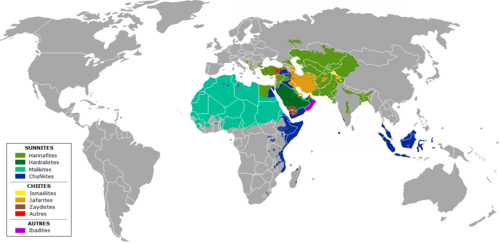
\includegraphics{Images/image097.png}
\vide{ruxe9ponse-soufie}{%
\subsection{Réponse soufie}\label{ruxe9ponse-soufie}}

Je vous propose de lire la lettre du Cheikh Ahmad al-Alawī
(1874-1934)~intitulée «~Lettre ouverte à celui qui critique le
soufisme~».

\vide{v--les-ordres-confruxe9riques}{%
\section{Les ordres
confrériques}\label{v--les-ordres-confruxe9riques}}

Il y en a une cinquantaine dans le monde.

\begin{itemize}
\item
  \textit{La qādirīya}
Fondateur~: `Abd al-Qādir al-Ğīlānī (m. 1166)
Implantation~: dans tous les pays musulmans, du Maghreb à la Chine


\item
  \textit{La Naqchabandīya}
Fondée au milieu du XIV° siècle
Implantation~: du Caucasse au Turkestan et à l'Inde
Elle a nourri le nationalisme kurde


\item
  \textit{La Šāḏilīya}
Eric Geoffroy dit de la \emph{Šāḏiliyya} qu'elle est l'une des
«~voies-mères~» du soufisme. Elle est apparue entre la fin du
XII\textsuperscript{e} siècle et le XIV\textsuperscript{e} siècle.
D'origine maghrébine, elle s'est diffusée au XIII\textsuperscript{e}
siècle, à partir de l'Égypte, dans la majeure partie du monde musulman.
Son enseignement est dense et il s'appuie sur les écrits d'Ibn
\emph{`}Arabī.
\end{itemize}
Toute voie initiatique a pour but de mener ses adeptes vers la sainteté,
ou «~proximité divine~» (\emph{walâya})~; celle-ci est identifiée au
plus haut degré de la gnose par al-Shâdhilî. De façon schématique, les
premiers maîtres shâdhilis distinguent deux niveaux~: la sainteté
«~mineure~» (\emph{sughrâ}), ouverte au public large des fidèles, et la
sainteté «~majeure~» (\emph{kubrâ}), réservée à une élite spirituelle.
Mais le terme \emph{walâya}, tout comme celui de sainteté en français,
est un terme générique, un idéal qui implique une méthode pour y
parvenir.

Pour les Shâdhilis, la réponse est claire~: c'est dans l'imitation
intérieure du Prophète que se réalise la \emph{walâya}. Réapparaît ici
le débat millénaire sur les rapports entre \emph{walâya}et
\emph{nubuwwa}, la prophétie, débats qui ont partagé exotéristes et
ésotéristes de l'islam, mais aussi les milieux soufis. Autant les
maîtres shâdhilis initiaux se réclament du premier théoricien de la
sainteté en islam, al-Hakîm al-Tirmidhî (m. 318/930), autant ils s'en
éloignent lorsque celui-ci accorde à la \emph{walâya}une autonomie par
rapport à la \emph{nubuwwa}~: pour eux, la première est subordonnée à la
seconde, et puise sa substance même dans la Lumière muhammadienne
(\emph{al-nûr al-muhammadî}).

\begin{itemize}
\item
  \textit{La Bekt'āchīya}
Elle impose le célibat
De nombreux affiliés en Turquie et Albanie


\item
  \textit{La Tidjānīya}
Influente au Maghreb et dans l'Afrique occidentale


\item
  \textit{La Chattārīya}
Influente en Inde et Malaisie

\item
  \textit{La Rah'mānīya}
La plus influente confrérie algérienne.


\item
  \textit{La mawlāwīya} (derviches)
\end{itemize}

Il existe plusieurs ordres soufis, mais l'on peut distinguer deux grands
groupes de mystiques~: ceux qui se trouvent dans la station de l'ivresse
(\emph{sukr}) et ceux qui sont dans la station de la sobriété
(\emph{sahw}).

Les initiés ivres sont souvent les disciples d'Abū Yazīd Bistamī (m.
875)~: l'ivresse, c'est la perte de sens commun, de la maîtrise de soi.
L'âme est enivrée de la connaissance de Dieu, plongée dans la
contemplation de Dieu.

Pour le second groupe, l'ivresse n'est qu'un état transitoire. Elle est
le début de l'unicité, mais elle se caractérise par la sobriété, quand
il sait que le soi n'est qu'un miroir dans lequel se réfléchit l'Essence
divine.

\paragraph{Pour aller plus loin}

Martin \textsc{Lings}, \emph{Qu'est-ce que le soufisme~?} traduit de
l'anglais par Roger du Pasquier, Paris, Éditions du Seuil, 1977.

Eric \textsc{Geoffroy},
«~\url{http://www.facebook.com/topic.php?uid=21148739744\&topic=3226}{L'islamité
du soufisme et son apport à la spiritualité universelle}~» dans
\url{http://www.religioperennis.org/documents/geoffroy/islamitesoufisme.pdf}

Eric \textsc{Geoffroy}, \emph{Initiation au soufisme}, Coll. L'espace
intérieur, Paris, Fayard, 2003.

Alberto Fabio \textsc{Ambrosio}, \emph{Vie d'un derviche tourneur}.
Doctrine et rituels du soufisme au XVII\textsuperscript{e} siècle,
Paris, CNRS Edition, 2010, 1 vol., 406 pages.

Laleh \textsc{Bakhtiar}, \emph{Le soufisme}. Expressions de la quête
mystique, Paris, Seuil, 1977.

Christian \textsc{Bonaud}, \emph{Le soufisme al-taṣawwuf et la
spiritualité islamique}, Préface de

Michel Chodkiewicz, Maison Larose, IMA, 1991.

\textbf{Exercice pour la Validation}

À partir de la lettre du šaḫy Ahmad al-Alawī, identifierez les éléments
qui répondent aux critiques adressées aux soufis et à Ibn `Arabī tels
que nous les avons exposés.


